\subsection{Consistency}
\label{sec:consistency}

\newcommand{\consis}{\mathcal{C}}


\begin{figure*}[!t]
    \vskip 0.2in
    \begin{center}
    \centering
    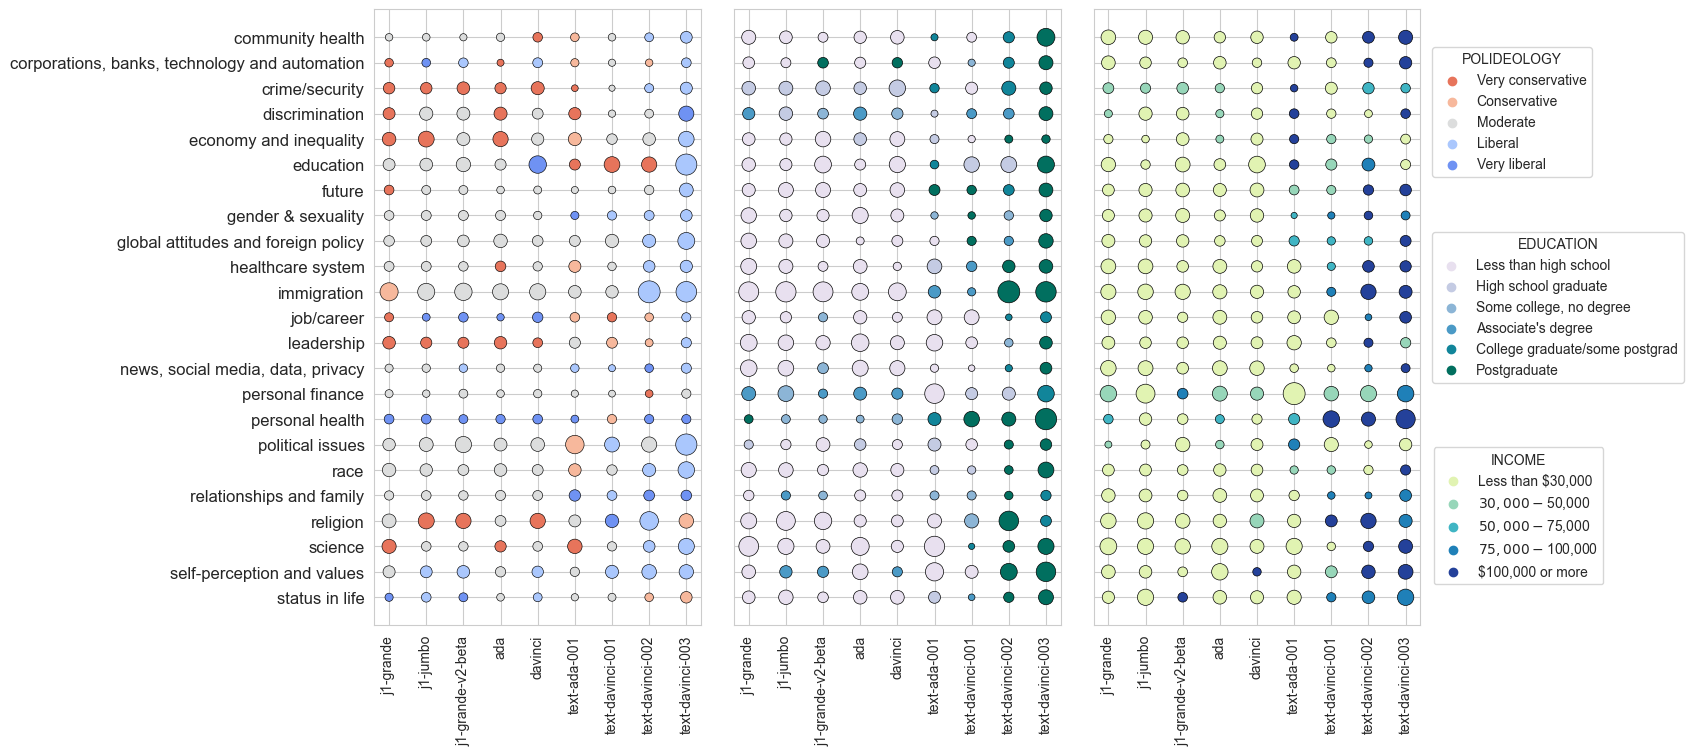
\includegraphics[width=1\textwidth]{Figures/consistency_cg.png}
    \caption{
      Consistency of different LMs (columns) across topics (rows) on different demographic attributes (panels). Each dot indicates an LM-topic pair, with the color indicating the group to which the model is best aligned, and the size of the dot indicates the strength of this alignment (computed as the ratio of the best and worst subgroup representativeness for that topic, see Appendix~\ref{app:consistency} for details). We find significant topic-level inconsistencies, especially for base LMs, and strong educational attainment consistency for RLHF trained LMs.}
    \label{fig:topic_ideology}
    \end{center}
    \vskip -0.2in
\end{figure*}



Our earlier default representativeness analysis (Section~\ref{sec:rep}) showed marked skews in the views expressed by LMs, with base LMs reflecting opinions consistent with lower income and education and the opposite for human-feedback tuned ones.
However, we might want to go beyond this aggregate analysis and ask:  \emph{are the views expressed by LMs consistent across topics?}~\citep{saris2004studies}.
For instance, is \model{text-davinci-002} politically Liberal on all matters or does it take a Conservative stance in some cases?
We now leverage the fine-grained topic taxonomy in our \bname dataset to answer this question.
To this end, we  inspect human-LM opinion similarity on a topic level by computing alignment on a subset of questions $Q_T$.



\paragraph{Are LMs consistent?}
In Figure~\ref{fig:topic_ideology}, we break down the subgroups that various LMs (columns) most closely align to (colors) across 23 topic categories (rows) by political ideology, education and income. 
Of all the LMs we study, the base models from both providers and the RLHF-trained \model{text-davinci-003} from OpenAI seem to be the most consistent -- albeit towards different sets of groups.
None of the models are perfectly consistent however, and even \model{text-davinci-00\{2,3\}} aligns with conservatives on topics like religion.

\paragraph{The metric.}
To distill these trends into a single measure, we ask what is the fraction of topics for which an LM's most aligned group overall (weighting topics equally) matches the LM's most aligned group on the given topic (with questions $Q_t$).
Specifically, for a model, we first identify the group it best aligns to across topics as 
\begin{equation*} 
  G_m^{best} := \argmax_{G} \left( \frac{1}{T} \sum_{T'}\mathcal{R}^{G}_M(Q_{T'}) \right)  
\end{equation*}
\noindent We then define consistency as:
\begin{equation*} 
\consis_m := \frac{1}{T}\sum_{T} \mathbbm{1} \left [ \left(\argmax_{G} \mathcal{R}^{G}_M(Q_T)\right)  = G_m^{best}  \right ] %
\end{equation*}
Our metric $\consis_m$ is bounded between 0 and 1, and a higher score implies that the model agrees with the views of the same subgroups across all topics.
In Figure~\ref{fig:inconsistency}, we visualize the average consistency score of a model across demographic traits (religion/income/ideology, etc). We find that the overall consistency scores of current LMs are fairly low---indicating that they are expressing a patchwork of disparate opinions.
Note that this may not always be problematic---after all even individuals can hold seemingly inconsistent beliefs.

\begin{figure*}[!t]
    \vskip 0.2in
    \begin{center}
    \centerline{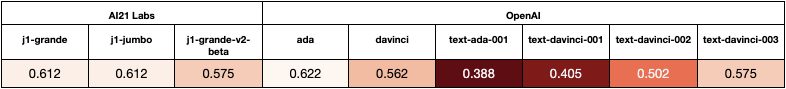
\includegraphics[width=0.95\textwidth]{Figures/consistency.png}}
      \caption{Consistency of LM opinions $\consis_m$, where a higher score (lighter) indicates that an LM aligns with the same set of groups across topics.
      }
    \label{fig:inconsistency}
    \end{center}
    \vskip -0.2in
\end{figure*}

















